\hypertarget{arrow_8h}{
\section{lib/arrow.h File Reference}
\label{arrow_8h}\index{lib/arrow.h@{lib/arrow.h}}
}
Header file for the Arrow callable library. 

{\tt \#include $<$stdio.h$>$}\par
{\tt \#include $<$stdlib.h$>$}\par
{\tt \#include $<$string.h$>$}\par
{\tt \#include $<$errno.h$>$}\par
{\tt \#include $<$limits.h$>$}\par
{\tt \#include $<$unistd.h$>$}\par
{\tt \#include \char`\"{}concorde.h\char`\"{}}\par


Include dependency graph for arrow.h:\nopagebreak
\begin{figure}[H]
\begin{center}
\leavevmode
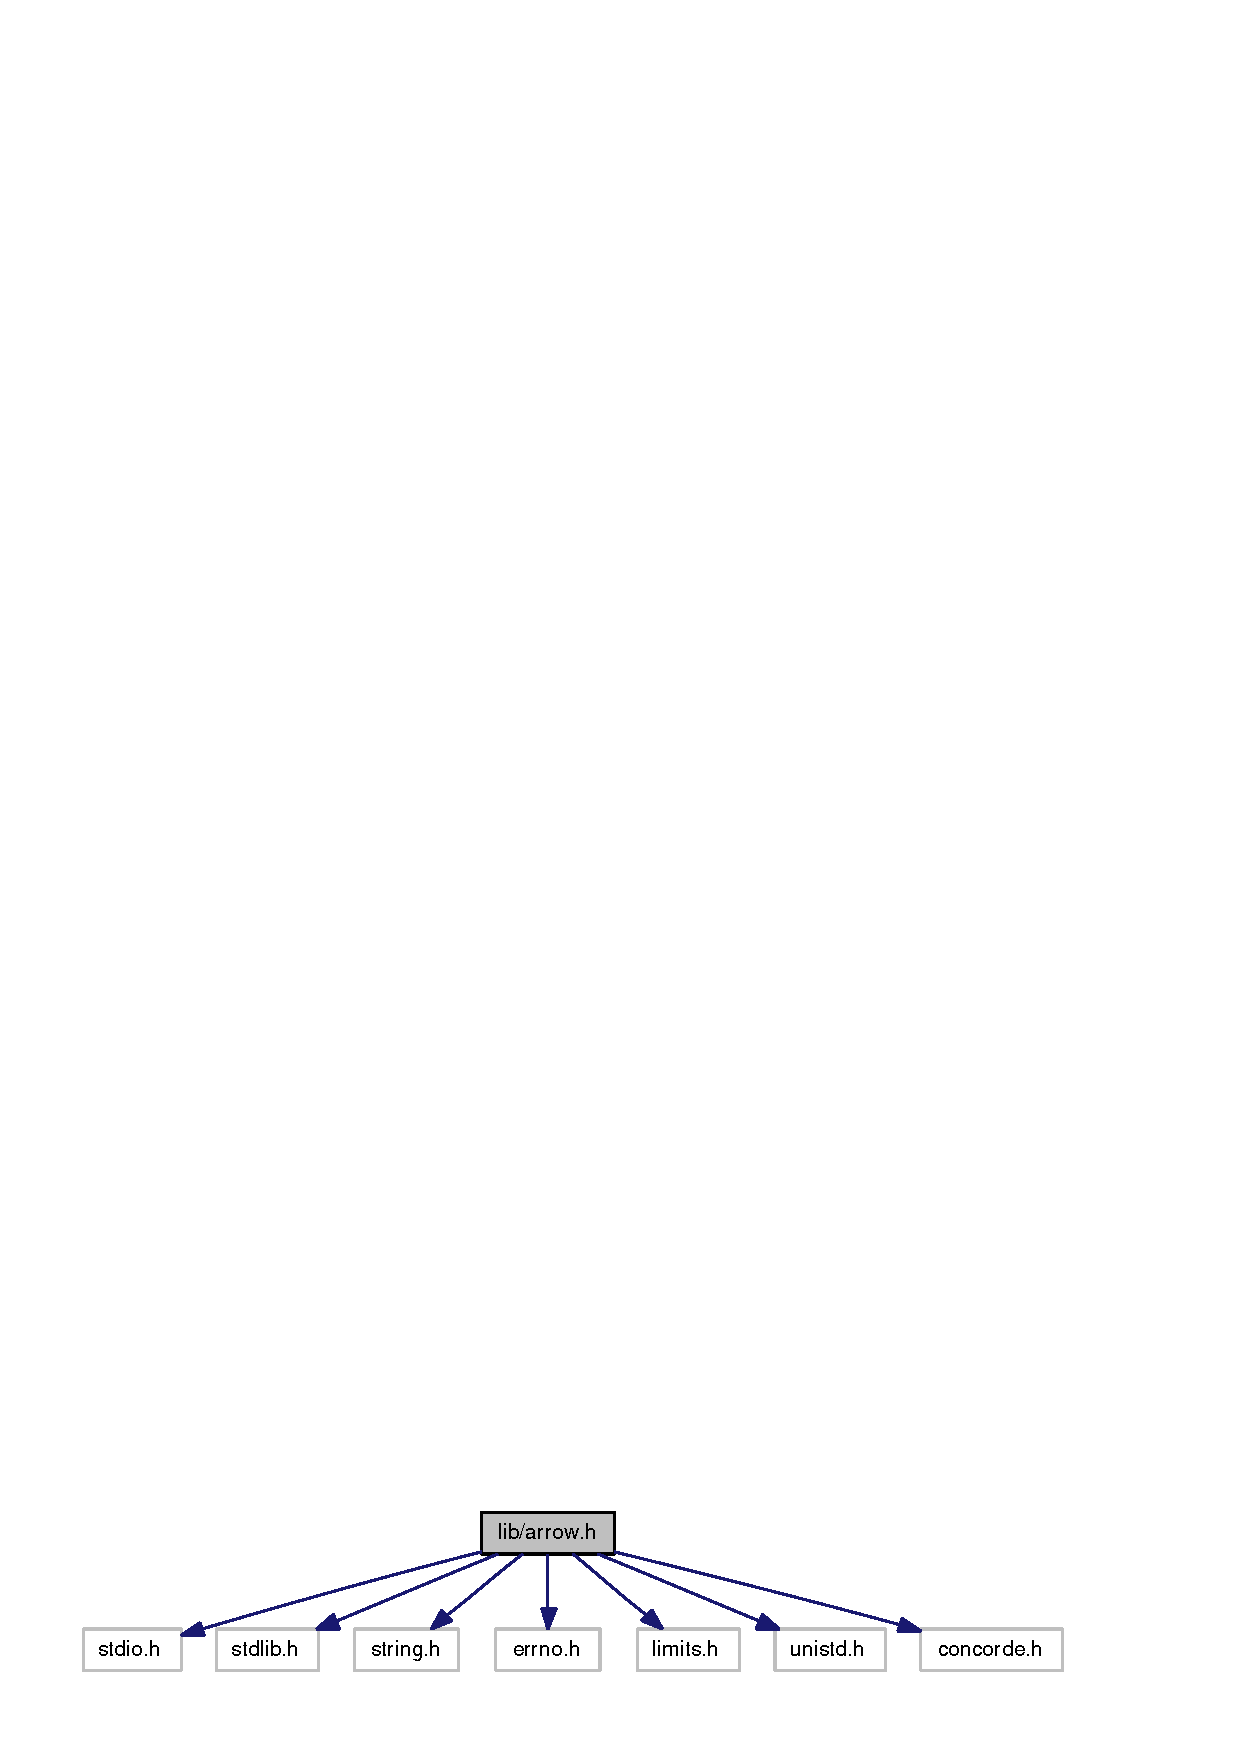
\includegraphics[width=257pt]{arrow_8h__incl}
\end{center}
\end{figure}


This graph shows which files directly or indirectly include this file:\nopagebreak
\begin{figure}[H]
\begin{center}
\leavevmode
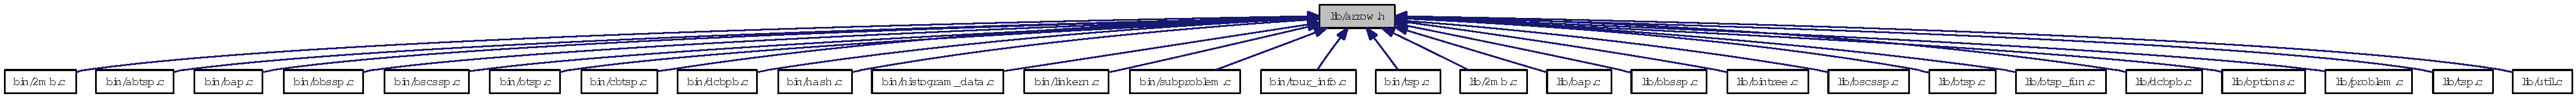
\includegraphics[width=319pt]{arrow_8h__dep__incl}
\end{center}
\end{figure}
\subsection*{Data Structures}
\begin{CompactItemize}
\item 
struct \hyperlink{structarrow__problem}{arrow\_\-problem}
\begin{CompactList}\small\item\em Problem data structure. \item\end{CompactList}\item 
struct \hyperlink{structarrow__problem__info}{arrow\_\-problem\_\-info}
\begin{CompactList}\small\item\em Problem information data structure. \item\end{CompactList}\item 
struct \hyperlink{structarrow__bintree}{arrow\_\-bintree}
\begin{CompactList}\small\item\em Binary tree data structure. \item\end{CompactList}\item 
struct \hyperlink{structarrow__bintree__node}{arrow\_\-bintree\_\-node}
\begin{CompactList}\small\item\em Binary tree node. \item\end{CompactList}\item 
struct \hyperlink{structarrow__bbssp__result}{arrow\_\-bbssp\_\-result}
\begin{CompactList}\small\item\em BBSSP solver result. \item\end{CompactList}\item 
struct \hyperlink{structarrow__tsp__result}{arrow\_\-tsp\_\-result}
\begin{CompactList}\small\item\em TSP result (including result from LK heuristic). \item\end{CompactList}\item 
struct \hyperlink{structarrow__tsp__lk__params}{arrow\_\-tsp\_\-lk\_\-params}
\begin{CompactList}\small\item\em LK algorithm parameters. \item\end{CompactList}\end{CompactItemize}
\subsection*{Defines}
\begin{CompactItemize}
\item 
\#define \hyperlink{arrow_8h_0be07738336b219a8057fb867ed386c1}{ARROW\_\-DEV\_\-NULL}~\char`\"{}/dev/null\char`\"{}
\item 
\#define \hyperlink{arrow_8h_21afcc3dc34f8488ad437841f58225c4}{ARROW\_\-SUCCESS}~1
\item 
\#define \hyperlink{arrow_8h_4a768d7e7c23ac0605a6e93ca16aaae2}{ARROW\_\-ERROR\_\-INPUT}~0
\item 
\#define \hyperlink{arrow_8h_3db3c8a03b898dcf83be87b8f8ef6419}{ARROW\_\-ERROR\_\-FATAL}~-1
\item 
\#define \hyperlink{arrow_8h_4635c151cf4dcc2f2ed67fed822bb51e}{ARROW\_\-ERROR\_\-NON\_\-FATAL}~-2
\item 
\#define \hyperlink{arrow_8h_42c447b913ad11889bf816691e423644}{ARROW\_\-TRUE}~1
\item 
\#define \hyperlink{arrow_8h_518134a9986d0e6bf31ec2480116ac76}{ARROW\_\-FALSE}~0
\item 
\#define \hyperlink{arrow_8h_2bc89592b4a27c03c1129b8e4b876a51}{arrow\_\-print\_\-error}(message)~arrow\_\-util\_\-print\_\-error(\_\-\_\-FILE\_\-\_\-, \_\-\_\-LINE\_\-\_\-, message)
\end{CompactItemize}
\subsection*{Functions}
\begin{CompactItemize}
\item 
int \hyperlink{arrow_8h_d6098d008ef724a58c6960d8f28bf925}{arrow\_\-bbssp\_\-solve} (\hyperlink{structarrow__problem}{arrow\_\-problem} $\ast$problem, \hyperlink{structarrow__problem__info}{arrow\_\-problem\_\-info} $\ast$info, \hyperlink{structarrow__bbssp__result}{arrow\_\-bbssp\_\-result} $\ast$result)
\begin{CompactList}\small\item\em Solves the bottleneck biconnected spanning subgraph problem (BBSSP) on the given problem. \item\end{CompactList}\item 
int \hyperlink{arrow_8h_727cb19dd9cfa6315e1155796daef833}{arrow\_\-bbssp\_\-biconnected} (\hyperlink{structarrow__problem}{arrow\_\-problem} $\ast$problem, int max\_\-cost, int $\ast$result)
\begin{CompactList}\small\item\em Determines if the graph is biconnected using only edges with costs less than or equal to the given value. \item\end{CompactList}\item 
void \hyperlink{arrow_8h_b28bc6559b228f0aa65cc671f67b9a09}{arrow\_\-bintree\_\-init} (\hyperlink{structarrow__bintree}{arrow\_\-bintree} $\ast$tree)
\begin{CompactList}\small\item\em Initializes the binary tree data structure. \item\end{CompactList}\item 
void \hyperlink{arrow_8h_ca9875422bf132eb9f5a4a2d10053207}{arrow\_\-bintree\_\-destruct} (\hyperlink{structarrow__bintree}{arrow\_\-bintree} $\ast$tree)
\begin{CompactList}\small\item\em Destructs a binary tree data structure. \item\end{CompactList}\item 
int \hyperlink{arrow_8h_75b4ee03b9667bd0e13e6cc71043e0a9}{arrow\_\-bintree\_\-insert} (\hyperlink{structarrow__bintree}{arrow\_\-bintree} $\ast$tree, int value)
\begin{CompactList}\small\item\em Inserts a value into the binary tree. \item\end{CompactList}\item 
int \hyperlink{arrow_8h_37fe2e7fbd64399611ba819ccfd5d4a2}{arrow\_\-bintree\_\-to\_\-array} (\hyperlink{structarrow__bintree}{arrow\_\-bintree} $\ast$tree, int $\ast$$\ast$array)
\begin{CompactList}\small\item\em Initializes the binary tree data structure. \item\end{CompactList}\item 
void \hyperlink{arrow_8h_3804a3bce6fc22ef6d5ea0ac5776a2bb}{arrow\_\-bintree\_\-print} (\hyperlink{structarrow__bintree}{arrow\_\-bintree} $\ast$tree)
\begin{CompactList}\small\item\em Prints out the values of the binary tree. \item\end{CompactList}\item 
int \hyperlink{arrow_8h_b5b9bae9f92630983d3b3d39d86198f8}{arrow\_\-problem\_\-read} (char $\ast$file\_\-name, \hyperlink{structarrow__problem}{arrow\_\-problem} $\ast$problem)
\begin{CompactList}\small\item\em Reads a problem from a TSPLIB file. \item\end{CompactList}\item 
void \hyperlink{arrow_8h_a702972ab510dcc6354d7679759611d1}{arrow\_\-problem\_\-destruct} (\hyperlink{structarrow__problem}{arrow\_\-problem} $\ast$problem)
\begin{CompactList}\small\item\em Deallocates problem data structure. \item\end{CompactList}\item 
int \hyperlink{arrow_8h_01623c45a7e1726ef7eeeec300e75bff}{arrow\_\-problem\_\-info\_\-get} (\hyperlink{structarrow__problem}{arrow\_\-problem} $\ast$problem, \hyperlink{structarrow__problem__info}{arrow\_\-problem\_\-info} $\ast$info)
\begin{CompactList}\small\item\em Builds ordered cost list and finds min/max cost in a problem. \item\end{CompactList}\item 
void \hyperlink{arrow_8h_09a5ba81556412e281fe6b863a6f08db}{arrow\_\-problem\_\-info\_\-destruct} (\hyperlink{structarrow__problem__info}{arrow\_\-problem\_\-info} $\ast$info)
\begin{CompactList}\small\item\em Deallocates problem info data structure. \item\end{CompactList}\item 
void \hyperlink{arrow_8h_ce6b857eab0a7a887262d033b7e5cf22}{arrow\_\-problem\_\-print} (\hyperlink{structarrow__problem}{arrow\_\-problem} $\ast$problem)
\begin{CompactList}\small\item\em Prints out information about a problem. \item\end{CompactList}\item 
void \hyperlink{arrow_8h_107b3fa0e8b3eeab9e04320d30654ec5}{arrow\_\-tsp\_\-result\_\-init} (\hyperlink{structarrow__problem}{arrow\_\-problem} $\ast$problem, \hyperlink{structarrow__tsp__result}{arrow\_\-tsp\_\-result} $\ast$result)
\begin{CompactList}\small\item\em Initializes the TSP result structure. \item\end{CompactList}\item 
void \hyperlink{arrow_8h_0665c82047dc78f8d08f12ecf5a9eef8}{arrow\_\-tsp\_\-result\_\-destruct} (\hyperlink{structarrow__tsp__result}{arrow\_\-tsp\_\-result} $\ast$result)
\begin{CompactList}\small\item\em Destructs a TSP result structure. \item\end{CompactList}\item 
void \hyperlink{arrow_8h_a20fdb653581bbcfcd08784900b19218}{arrow\_\-tsp\_\-lk\_\-params\_\-default} (\hyperlink{structarrow__problem}{arrow\_\-problem} $\ast$problem, \hyperlink{structarrow__tsp__lk__params}{arrow\_\-tsp\_\-lk\_\-params} $\ast$params)
\begin{CompactList}\small\item\em Sets default parameters for Lin-Kernighan heuristic:\begin{itemize}
\item stall\_\-count = problem-$>$size\item kicks = 0\item kick\_\-type = CC\_\-LK\_\-GEOMETRIC\_\-KICK\item time\_\-bound = 0.0\item length\_\-bound = 0.0\item initial\_\-tour = NULL. \end{itemize}
\item\end{CompactList}\item 
int \hyperlink{arrow_8h_0cc68200bf38d20fe0dd3c388674d215}{arrow\_\-tsp\_\-exact\_\-solve} (\hyperlink{structarrow__problem}{arrow\_\-problem} $\ast$problem, int $\ast$in\_\-tour, \hyperlink{structarrow__tsp__result}{arrow\_\-tsp\_\-result} $\ast$result)
\begin{CompactList}\small\item\em Solves TSP with Concorde's exact solver. \item\end{CompactList}\item 
int \hyperlink{arrow_8h_4aea68dfc908d08522baccb148251ae7}{arrow\_\-util\_\-create\_\-int\_\-array} (int size, int $\ast$$\ast$array)
\begin{CompactList}\small\item\em Creates an integer array. \item\end{CompactList}\item 
void \hyperlink{arrow_8h_3bd7042ebd6e97b5790a8708c91be5b4}{arrow\_\-util\_\-print\_\-error} (const char $\ast$file\_\-name, int line\_\-num, const char $\ast$message)
\begin{CompactList}\small\item\em Prints an error message to stderr with consistent formatting. \item\end{CompactList}\item 
double \hyperlink{arrow_8h_05b2e96c9991c51368c1f8d5a77d3ccf}{arrow\_\-util\_\-zeit} ()
\begin{CompactList}\small\item\em Used to measure timings. \item\end{CompactList}\item 
void \hyperlink{arrow_8h_8a9cef270a8d9d4fb22483dc986aa792}{arrow\_\-util\_\-redirect\_\-stdout\_\-to\_\-file} (const char $\ast$filename, int $\ast$old\_\-stream)
\begin{CompactList}\small\item\em Redirects STDOUT stream to a file (can be used to completely surpress output by directing to /dev/null). \item\end{CompactList}\item 
void \hyperlink{arrow_8h_65b9ba02b0c557fe9b15f5315a6953db}{arrow\_\-util\_\-restore\_\-stdout} (int old\_\-stream)
\begin{CompactList}\small\item\em Restores STDOUT stream that's been redirected. \item\end{CompactList}\end{CompactItemize}


\subsection{Detailed Description}
Header file for the Arrow callable library. 

Function prototypes and structures exposed by the callable library.

\begin{Desc}
\item[Author:]John LaRusic \end{Desc}


Definition in file \hyperlink{arrow_8h-source}{arrow.h}.

\subsection{Define Documentation}
\hypertarget{arrow_8h_0be07738336b219a8057fb867ed386c1}{
\index{arrow.h@{arrow.h}!ARROW\_\-DEV\_\-NULL@{ARROW\_\-DEV\_\-NULL}}
\index{ARROW\_\-DEV\_\-NULL@{ARROW\_\-DEV\_\-NULL}!arrow.h@{arrow.h}}
\subsubsection{\setlength{\rightskip}{0pt plus 5cm}\#define ARROW\_\-DEV\_\-NULL~\char`\"{}/dev/null\char`\"{}}}
\label{arrow_8h_0be07738336b219a8057fb867ed386c1}




Definition at line 24 of file arrow.h.

Referenced by main().\hypertarget{arrow_8h_3db3c8a03b898dcf83be87b8f8ef6419}{
\index{arrow.h@{arrow.h}!ARROW\_\-ERROR\_\-FATAL@{ARROW\_\-ERROR\_\-FATAL}}
\index{ARROW\_\-ERROR\_\-FATAL@{ARROW\_\-ERROR\_\-FATAL}!arrow.h@{arrow.h}}
\subsubsection{\setlength{\rightskip}{0pt plus 5cm}\#define ARROW\_\-ERROR\_\-FATAL~-1}}
\label{arrow_8h_3db3c8a03b898dcf83be87b8f8ef6419}




Definition at line 27 of file arrow.h.

Referenced by arrow\_\-bbssp\_\-biconnected(), arrow\_\-bbssp\_\-solve(), arrow\_\-problem\_\-read(), arrow\_\-tsp\_\-exact\_\-solve(), arrow\_\-util\_\-create\_\-int\_\-array(), construct\_\-node(), and insert\_\-at().\hypertarget{arrow_8h_4a768d7e7c23ac0605a6e93ca16aaae2}{
\index{arrow.h@{arrow.h}!ARROW\_\-ERROR\_\-INPUT@{ARROW\_\-ERROR\_\-INPUT}}
\index{ARROW\_\-ERROR\_\-INPUT@{ARROW\_\-ERROR\_\-INPUT}!arrow.h@{arrow.h}}
\subsubsection{\setlength{\rightskip}{0pt plus 5cm}\#define ARROW\_\-ERROR\_\-INPUT~0}}
\label{arrow_8h_4a768d7e7c23ac0605a6e93ca16aaae2}




Definition at line 26 of file arrow.h.\hypertarget{arrow_8h_4635c151cf4dcc2f2ed67fed822bb51e}{
\index{arrow.h@{arrow.h}!ARROW\_\-ERROR\_\-NON\_\-FATAL@{ARROW\_\-ERROR\_\-NON\_\-FATAL}}
\index{ARROW\_\-ERROR\_\-NON\_\-FATAL@{ARROW\_\-ERROR\_\-NON\_\-FATAL}!arrow.h@{arrow.h}}
\subsubsection{\setlength{\rightskip}{0pt plus 5cm}\#define ARROW\_\-ERROR\_\-NON\_\-FATAL~-2}}
\label{arrow_8h_4635c151cf4dcc2f2ed67fed822bb51e}




Definition at line 28 of file arrow.h.

Referenced by arrow\_\-tsp\_\-exact\_\-solve().\hypertarget{arrow_8h_518134a9986d0e6bf31ec2480116ac76}{
\index{arrow.h@{arrow.h}!ARROW\_\-FALSE@{ARROW\_\-FALSE}}
\index{ARROW\_\-FALSE@{ARROW\_\-FALSE}!arrow.h@{arrow.h}}
\subsubsection{\setlength{\rightskip}{0pt plus 5cm}\#define ARROW\_\-FALSE~0}}
\label{arrow_8h_518134a9986d0e6bf31ec2480116ac76}




Definition at line 30 of file arrow.h.

Referenced by arrow\_\-bbssp\_\-biconnected(), arrow\_\-problem\_\-read(), arrow\_\-tsp\_\-result\_\-init(), construct\_\-node(), and insert\_\-at().\hypertarget{arrow_8h_2bc89592b4a27c03c1129b8e4b876a51}{
\index{arrow.h@{arrow.h}!arrow\_\-print\_\-error@{arrow\_\-print\_\-error}}
\index{arrow\_\-print\_\-error@{arrow\_\-print\_\-error}!arrow.h@{arrow.h}}
\subsubsection{\setlength{\rightskip}{0pt plus 5cm}\#define arrow\_\-print\_\-error(message)~arrow\_\-util\_\-print\_\-error(\_\-\_\-FILE\_\-\_\-, \_\-\_\-LINE\_\-\_\-, message)}}
\label{arrow_8h_2bc89592b4a27c03c1129b8e4b876a51}




Definition at line 36 of file arrow.h.

Referenced by arrow\_\-util\_\-create\_\-int\_\-array(), construct\_\-node(), main(), and read\_\-args().\hypertarget{arrow_8h_21afcc3dc34f8488ad437841f58225c4}{
\index{arrow.h@{arrow.h}!ARROW\_\-SUCCESS@{ARROW\_\-SUCCESS}}
\index{ARROW\_\-SUCCESS@{ARROW\_\-SUCCESS}!arrow.h@{arrow.h}}
\subsubsection{\setlength{\rightskip}{0pt plus 5cm}\#define ARROW\_\-SUCCESS~1}}
\label{arrow_8h_21afcc3dc34f8488ad437841f58225c4}




Definition at line 25 of file arrow.h.

Referenced by arrow\_\-bbssp\_\-solve(), arrow\_\-bintree\_\-to\_\-array(), arrow\_\-problem\_\-info\_\-get(), arrow\_\-problem\_\-read(), arrow\_\-tsp\_\-exact\_\-solve(), arrow\_\-util\_\-create\_\-int\_\-array(), construct\_\-node(), find\_\-art\_\-points(), and insert\_\-at().\hypertarget{arrow_8h_42c447b913ad11889bf816691e423644}{
\index{arrow.h@{arrow.h}!ARROW\_\-TRUE@{ARROW\_\-TRUE}}
\index{ARROW\_\-TRUE@{ARROW\_\-TRUE}!arrow.h@{arrow.h}}
\subsubsection{\setlength{\rightskip}{0pt plus 5cm}\#define ARROW\_\-TRUE~1}}
\label{arrow_8h_42c447b913ad11889bf816691e423644}




Definition at line 29 of file arrow.h.

Referenced by arrow\_\-bbssp\_\-biconnected(), arrow\_\-bbssp\_\-solve(), destruct\_\-node(), insert\_\-at(), and read\_\-args().

\subsection{Function Documentation}
\hypertarget{arrow_8h_727cb19dd9cfa6315e1155796daef833}{
\index{arrow.h@{arrow.h}!arrow\_\-bbssp\_\-biconnected@{arrow\_\-bbssp\_\-biconnected}}
\index{arrow\_\-bbssp\_\-biconnected@{arrow\_\-bbssp\_\-biconnected}!arrow.h@{arrow.h}}
\subsubsection{\setlength{\rightskip}{0pt plus 5cm}int arrow\_\-bbssp\_\-biconnected ({\bf arrow\_\-problem} $\ast$ {\em problem}, \/  int {\em max\_\-cost}, \/  int $\ast$ {\em result})}}
\label{arrow_8h_727cb19dd9cfa6315e1155796daef833}


Determines if the graph is biconnected using only edges with costs less than or equal to the given value. 

\begin{Desc}
\item[Parameters:]
\begin{description}
\item[{\em problem}]\mbox{[}in\mbox{]} problem data \item[{\em max\_\-cost}]\mbox{[}in\mbox{]} value to check biconnectivity question against \item[{\em result}]\mbox{[}out\mbox{]} ARROW\_\-TRUE if biconnected, ARROW\_\-FALSE otherwise. \end{description}
\end{Desc}


Definition at line 88 of file bbssp.c.

References ARROW\_\-ERROR\_\-FATAL, ARROW\_\-FALSE, ARROW\_\-TRUE, arrow\_\-util\_\-create\_\-int\_\-array(), find\_\-art\_\-points(), and arrow\_\-problem::size.

Referenced by arrow\_\-bbssp\_\-solve().\hypertarget{arrow_8h_d6098d008ef724a58c6960d8f28bf925}{
\index{arrow.h@{arrow.h}!arrow\_\-bbssp\_\-solve@{arrow\_\-bbssp\_\-solve}}
\index{arrow\_\-bbssp\_\-solve@{arrow\_\-bbssp\_\-solve}!arrow.h@{arrow.h}}
\subsubsection{\setlength{\rightskip}{0pt plus 5cm}int arrow\_\-bbssp\_\-solve ({\bf arrow\_\-problem} $\ast$ {\em problem}, \/  {\bf arrow\_\-problem\_\-info} $\ast$ {\em info}, \/  {\bf arrow\_\-bbssp\_\-result} $\ast$ {\em result})}}
\label{arrow_8h_d6098d008ef724a58c6960d8f28bf925}


Solves the bottleneck biconnected spanning subgraph problem (BBSSP) on the given problem. 

\begin{Desc}
\item[Parameters:]
\begin{description}
\item[{\em problem}]\mbox{[}in\mbox{]} problem data \item[{\em result}]\mbox{[}out\mbox{]} BBSSP solution \end{description}
\end{Desc}


Definition at line 44 of file bbssp.c.

References arrow\_\-bbssp\_\-biconnected(), ARROW\_\-ERROR\_\-FATAL, ARROW\_\-SUCCESS, ARROW\_\-TRUE, arrow\_\-util\_\-zeit(), arrow\_\-problem\_\-info::cost\_\-list, arrow\_\-problem\_\-info::cost\_\-list\_\-length, arrow\_\-bbssp\_\-result::obj\_\-value, and arrow\_\-bbssp\_\-result::total\_\-time.

Referenced by main().\hypertarget{arrow_8h_ca9875422bf132eb9f5a4a2d10053207}{
\index{arrow.h@{arrow.h}!arrow\_\-bintree\_\-destruct@{arrow\_\-bintree\_\-destruct}}
\index{arrow\_\-bintree\_\-destruct@{arrow\_\-bintree\_\-destruct}!arrow.h@{arrow.h}}
\subsubsection{\setlength{\rightskip}{0pt plus 5cm}void arrow\_\-bintree\_\-destruct ({\bf arrow\_\-bintree} $\ast$ {\em tree})}}
\label{arrow_8h_ca9875422bf132eb9f5a4a2d10053207}


Destructs a binary tree data structure. 

\begin{Desc}
\item[Parameters:]
\begin{description}
\item[{\em tree}]\mbox{[}out\mbox{]} binary tree structure \end{description}
\end{Desc}


Definition at line 59 of file bintree.c.

References destruct\_\-node(), arrow\_\-bintree::root\_\-node, and arrow\_\-bintree::size.

Referenced by arrow\_\-problem\_\-info\_\-get().\hypertarget{arrow_8h_b28bc6559b228f0aa65cc671f67b9a09}{
\index{arrow.h@{arrow.h}!arrow\_\-bintree\_\-init@{arrow\_\-bintree\_\-init}}
\index{arrow\_\-bintree\_\-init@{arrow\_\-bintree\_\-init}!arrow.h@{arrow.h}}
\subsubsection{\setlength{\rightskip}{0pt plus 5cm}void arrow\_\-bintree\_\-init ({\bf arrow\_\-bintree} $\ast$ {\em tree})}}
\label{arrow_8h_b28bc6559b228f0aa65cc671f67b9a09}


Initializes the binary tree data structure. 

\begin{Desc}
\item[Parameters:]
\begin{description}
\item[{\em tree}]\mbox{[}out\mbox{]} binary tree structure \end{description}
\end{Desc}


Definition at line 52 of file bintree.c.

References arrow\_\-bintree::root\_\-node, and arrow\_\-bintree::size.

Referenced by arrow\_\-problem\_\-info\_\-get().\hypertarget{arrow_8h_75b4ee03b9667bd0e13e6cc71043e0a9}{
\index{arrow.h@{arrow.h}!arrow\_\-bintree\_\-insert@{arrow\_\-bintree\_\-insert}}
\index{arrow\_\-bintree\_\-insert@{arrow\_\-bintree\_\-insert}!arrow.h@{arrow.h}}
\subsubsection{\setlength{\rightskip}{0pt plus 5cm}int arrow\_\-bintree\_\-insert ({\bf arrow\_\-bintree} $\ast$ {\em tree}, \/  int {\em value})}}
\label{arrow_8h_75b4ee03b9667bd0e13e6cc71043e0a9}


Inserts a value into the binary tree. 

\begin{Desc}
\item[Parameters:]
\begin{description}
\item[{\em tree}]\mbox{[}out\mbox{]} binary tree structure \item[{\em value}]\mbox{[}in\mbox{]} value to insert into tree \end{description}
\end{Desc}


Definition at line 66 of file bintree.c.

References construct\_\-node(), insert\_\-at(), arrow\_\-bintree::root\_\-node, and arrow\_\-bintree::size.

Referenced by arrow\_\-problem\_\-info\_\-get().\hypertarget{arrow_8h_3804a3bce6fc22ef6d5ea0ac5776a2bb}{
\index{arrow.h@{arrow.h}!arrow\_\-bintree\_\-print@{arrow\_\-bintree\_\-print}}
\index{arrow\_\-bintree\_\-print@{arrow\_\-bintree\_\-print}!arrow.h@{arrow.h}}
\subsubsection{\setlength{\rightskip}{0pt plus 5cm}void arrow\_\-bintree\_\-print ({\bf arrow\_\-bintree} $\ast$ {\em tree})}}
\label{arrow_8h_3804a3bce6fc22ef6d5ea0ac5776a2bb}


Prints out the values of the binary tree. 

\begin{Desc}
\item[Parameters:]
\begin{description}
\item[{\em tree}]\mbox{[}in\mbox{]} binary tree structure \end{description}
\end{Desc}
\hypertarget{arrow_8h_37fe2e7fbd64399611ba819ccfd5d4a2}{
\index{arrow.h@{arrow.h}!arrow\_\-bintree\_\-to\_\-array@{arrow\_\-bintree\_\-to\_\-array}}
\index{arrow\_\-bintree\_\-to\_\-array@{arrow\_\-bintree\_\-to\_\-array}!arrow.h@{arrow.h}}
\subsubsection{\setlength{\rightskip}{0pt plus 5cm}int arrow\_\-bintree\_\-to\_\-array ({\bf arrow\_\-bintree} $\ast$ {\em tree}, \/  int $\ast$$\ast$ {\em array})}}
\label{arrow_8h_37fe2e7fbd64399611ba819ccfd5d4a2}


Initializes the binary tree data structure. 

\begin{Desc}
\item[Parameters:]
\begin{description}
\item[{\em tree}]\mbox{[}out\mbox{]} binary tree structure \item[{\em array}]\mbox{[}out\mbox{]} array to be created and filled \end{description}
\end{Desc}


Definition at line 86 of file bintree.c.

References ARROW\_\-SUCCESS, arrow\_\-util\_\-create\_\-int\_\-array(), fill\_\-array(), arrow\_\-bintree::root\_\-node, and arrow\_\-bintree::size.

Referenced by arrow\_\-problem\_\-info\_\-get().\hypertarget{arrow_8h_a702972ab510dcc6354d7679759611d1}{
\index{arrow.h@{arrow.h}!arrow\_\-problem\_\-destruct@{arrow\_\-problem\_\-destruct}}
\index{arrow\_\-problem\_\-destruct@{arrow\_\-problem\_\-destruct}!arrow.h@{arrow.h}}
\subsubsection{\setlength{\rightskip}{0pt plus 5cm}void arrow\_\-problem\_\-destruct ({\bf arrow\_\-problem} $\ast$ {\em problem})}}
\label{arrow_8h_a702972ab510dcc6354d7679759611d1}


Deallocates problem data structure. 

\begin{Desc}
\item[Parameters:]
\begin{description}
\item[{\em problem}]\mbox{[}in\mbox{]} problem data structure \end{description}
\end{Desc}


Definition at line 50 of file problem.c.

References arrow\_\-problem::data.

Referenced by main().\hypertarget{arrow_8h_09a5ba81556412e281fe6b863a6f08db}{
\index{arrow.h@{arrow.h}!arrow\_\-problem\_\-info\_\-destruct@{arrow\_\-problem\_\-info\_\-destruct}}
\index{arrow\_\-problem\_\-info\_\-destruct@{arrow\_\-problem\_\-info\_\-destruct}!arrow.h@{arrow.h}}
\subsubsection{\setlength{\rightskip}{0pt plus 5cm}void arrow\_\-problem\_\-info\_\-destruct ({\bf arrow\_\-problem\_\-info} $\ast$ {\em info})}}
\label{arrow_8h_09a5ba81556412e281fe6b863a6f08db}


Deallocates problem info data structure. 

\begin{Desc}
\item[Parameters:]
\begin{description}
\item[{\em info}]\mbox{[}in\mbox{]} problem info data structure \end{description}
\end{Desc}


Definition at line 99 of file problem.c.

References arrow\_\-problem\_\-info::cost\_\-list.

Referenced by main().\hypertarget{arrow_8h_01623c45a7e1726ef7eeeec300e75bff}{
\index{arrow.h@{arrow.h}!arrow\_\-problem\_\-info\_\-get@{arrow\_\-problem\_\-info\_\-get}}
\index{arrow\_\-problem\_\-info\_\-get@{arrow\_\-problem\_\-info\_\-get}!arrow.h@{arrow.h}}
\subsubsection{\setlength{\rightskip}{0pt plus 5cm}int arrow\_\-problem\_\-info\_\-get ({\bf arrow\_\-problem} $\ast$ {\em problem}, \/  {\bf arrow\_\-problem\_\-info} $\ast$ {\em info})}}
\label{arrow_8h_01623c45a7e1726ef7eeeec300e75bff}


Builds ordered cost list and finds min/max cost in a problem. 

\begin{Desc}
\item[Parameters:]
\begin{description}
\item[{\em problem}]\mbox{[}in\mbox{]} problem data structure \item[{\em info}]\mbox{[}out\mbox{]} problem info data structure \end{description}
\end{Desc}


Definition at line 60 of file problem.c.

References arrow\_\-bintree\_\-destruct(), arrow\_\-bintree\_\-init(), arrow\_\-bintree\_\-insert(), arrow\_\-bintree\_\-to\_\-array(), ARROW\_\-SUCCESS, arrow\_\-problem\_\-info::cost\_\-list, arrow\_\-problem\_\-info::cost\_\-list\_\-length, arrow\_\-problem::get\_\-cost, arrow\_\-problem\_\-info::max\_\-cost, arrow\_\-problem\_\-info::min\_\-cost, arrow\_\-bintree::size, and arrow\_\-problem::size.

Referenced by main().\hypertarget{arrow_8h_ce6b857eab0a7a887262d033b7e5cf22}{
\index{arrow.h@{arrow.h}!arrow\_\-problem\_\-print@{arrow\_\-problem\_\-print}}
\index{arrow\_\-problem\_\-print@{arrow\_\-problem\_\-print}!arrow.h@{arrow.h}}
\subsubsection{\setlength{\rightskip}{0pt plus 5cm}void arrow\_\-problem\_\-print ({\bf arrow\_\-problem} $\ast$ {\em problem})}}
\label{arrow_8h_ce6b857eab0a7a887262d033b7e5cf22}


Prints out information about a problem. 

\begin{Desc}
\item[Parameters:]
\begin{description}
\item[{\em problem}]\mbox{[}in\mbox{]} problem data structure \end{description}
\end{Desc}


Definition at line 106 of file problem.c.

References arrow\_\-problem::get\_\-cost, and arrow\_\-problem::size.\hypertarget{arrow_8h_b5b9bae9f92630983d3b3d39d86198f8}{
\index{arrow.h@{arrow.h}!arrow\_\-problem\_\-read@{arrow\_\-problem\_\-read}}
\index{arrow\_\-problem\_\-read@{arrow\_\-problem\_\-read}!arrow.h@{arrow.h}}
\subsubsection{\setlength{\rightskip}{0pt plus 5cm}int arrow\_\-problem\_\-read (char $\ast$ {\em file\_\-name}, \/  {\bf arrow\_\-problem} $\ast$ {\em problem})}}
\label{arrow_8h_b5b9bae9f92630983d3b3d39d86198f8}


Reads a problem from a TSPLIB file. 

\begin{Desc}
\item[Parameters:]
\begin{description}
\item[{\em file\_\-name}]\mbox{[}in\mbox{]} path to TSPLIB file \item[{\em problem}]\mbox{[}out\mbox{]} problem data structure \end{description}
\end{Desc}


Definition at line 30 of file problem.c.

References ARROW\_\-ERROR\_\-FATAL, ARROW\_\-FALSE, ARROW\_\-SUCCESS, concorde\_\-get\_\-cost(), arrow\_\-problem::data, arrow\_\-problem::get\_\-cost, arrow\_\-problem::name, arrow\_\-problem::shallow, and arrow\_\-problem::size.

Referenced by main().\hypertarget{arrow_8h_0cc68200bf38d20fe0dd3c388674d215}{
\index{arrow.h@{arrow.h}!arrow\_\-tsp\_\-exact\_\-solve@{arrow\_\-tsp\_\-exact\_\-solve}}
\index{arrow\_\-tsp\_\-exact\_\-solve@{arrow\_\-tsp\_\-exact\_\-solve}!arrow.h@{arrow.h}}
\subsubsection{\setlength{\rightskip}{0pt plus 5cm}int arrow\_\-tsp\_\-exact\_\-solve ({\bf arrow\_\-problem} $\ast$ {\em problem}, \/  int $\ast$ {\em in\_\-tour}, \/  {\bf arrow\_\-tsp\_\-result} $\ast$ {\em result})}}
\label{arrow_8h_0cc68200bf38d20fe0dd3c388674d215}


Solves TSP with Concorde's exact solver. 

\begin{Desc}
\item[Parameters:]
\begin{description}
\item[{\em problem}]\mbox{[}in\mbox{]} problem to solve \item[{\em in\_\-tour}]\mbox{[}in\mbox{]} an initial tour (can be NULL) \item[{\em result}]\mbox{[}out\mbox{]} TSP solution \end{description}
\end{Desc}


Definition at line 36 of file tsp.c.

References ARROW\_\-ERROR\_\-FATAL, ARROW\_\-ERROR\_\-NON\_\-FATAL, ARROW\_\-SUCCESS, arrow\_\-util\_\-zeit(), arrow\_\-problem::data, arrow\_\-tsp\_\-result::found\_\-tour, arrow\_\-problem::name, arrow\_\-problem::size, arrow\_\-tsp\_\-result::total\_\-time, arrow\_\-tsp\_\-result::tour, and arrow\_\-tsp\_\-result::tour\_\-length.\hypertarget{arrow_8h_a20fdb653581bbcfcd08784900b19218}{
\index{arrow.h@{arrow.h}!arrow\_\-tsp\_\-lk\_\-params\_\-default@{arrow\_\-tsp\_\-lk\_\-params\_\-default}}
\index{arrow\_\-tsp\_\-lk\_\-params\_\-default@{arrow\_\-tsp\_\-lk\_\-params\_\-default}!arrow.h@{arrow.h}}
\subsubsection{\setlength{\rightskip}{0pt plus 5cm}void arrow\_\-tsp\_\-lk\_\-params\_\-default ({\bf arrow\_\-problem} $\ast$ {\em problem}, \/  {\bf arrow\_\-tsp\_\-lk\_\-params} $\ast$ {\em params})}}
\label{arrow_8h_a20fdb653581bbcfcd08784900b19218}


Sets default parameters for Lin-Kernighan heuristic:\begin{itemize}
\item stall\_\-count = problem-$>$size\item kicks = 0\item kick\_\-type = CC\_\-LK\_\-GEOMETRIC\_\-KICK\item time\_\-bound = 0.0\item length\_\-bound = 0.0\item initial\_\-tour = NULL. \end{itemize}


\begin{Desc}
\item[Parameters:]
\begin{description}
\item[{\em problem}]\mbox{[}in\mbox{]} problem to solve \item[{\em params}]\mbox{[}out\mbox{]} LK parameters structure \end{description}
\end{Desc}


Definition at line 29 of file tsp.c.\hypertarget{arrow_8h_0665c82047dc78f8d08f12ecf5a9eef8}{
\index{arrow.h@{arrow.h}!arrow\_\-tsp\_\-result\_\-destruct@{arrow\_\-tsp\_\-result\_\-destruct}}
\index{arrow\_\-tsp\_\-result\_\-destruct@{arrow\_\-tsp\_\-result\_\-destruct}!arrow.h@{arrow.h}}
\subsubsection{\setlength{\rightskip}{0pt plus 5cm}void arrow\_\-tsp\_\-result\_\-destruct ({\bf arrow\_\-tsp\_\-result} $\ast$ {\em result})}}
\label{arrow_8h_0665c82047dc78f8d08f12ecf5a9eef8}


Destructs a TSP result structure. 

\begin{Desc}
\item[Parameters:]
\begin{description}
\item[{\em result}]\mbox{[}out\mbox{]} TSP result structure \end{description}
\end{Desc}


Definition at line 22 of file tsp.c.

References arrow\_\-tsp\_\-result::tour.\hypertarget{arrow_8h_107b3fa0e8b3eeab9e04320d30654ec5}{
\index{arrow.h@{arrow.h}!arrow\_\-tsp\_\-result\_\-init@{arrow\_\-tsp\_\-result\_\-init}}
\index{arrow\_\-tsp\_\-result\_\-init@{arrow\_\-tsp\_\-result\_\-init}!arrow.h@{arrow.h}}
\subsubsection{\setlength{\rightskip}{0pt plus 5cm}void arrow\_\-tsp\_\-result\_\-init ({\bf arrow\_\-problem} $\ast$ {\em problem}, \/  {\bf arrow\_\-tsp\_\-result} $\ast$ {\em result})}}
\label{arrow_8h_107b3fa0e8b3eeab9e04320d30654ec5}


Initializes the TSP result structure. 

\begin{Desc}
\item[Parameters:]
\begin{description}
\item[{\em problem}]\mbox{[}in\mbox{]} problem to solve \item[{\em result}]\mbox{[}out\mbox{]} TSP result structure \end{description}
\end{Desc}


Definition at line 12 of file tsp.c.

References ARROW\_\-FALSE, arrow\_\-util\_\-create\_\-int\_\-array(), arrow\_\-tsp\_\-result::found\_\-tour, arrow\_\-problem::size, arrow\_\-tsp\_\-result::total\_\-time, arrow\_\-tsp\_\-result::tour, and arrow\_\-tsp\_\-result::tour\_\-length.\hypertarget{arrow_8h_4aea68dfc908d08522baccb148251ae7}{
\index{arrow.h@{arrow.h}!arrow\_\-util\_\-create\_\-int\_\-array@{arrow\_\-util\_\-create\_\-int\_\-array}}
\index{arrow\_\-util\_\-create\_\-int\_\-array@{arrow\_\-util\_\-create\_\-int\_\-array}!arrow.h@{arrow.h}}
\subsubsection{\setlength{\rightskip}{0pt plus 5cm}int arrow\_\-util\_\-create\_\-int\_\-array (int {\em size}, \/  int $\ast$$\ast$ {\em array})\hspace{0.3cm}{\tt  \mbox{[}inline\mbox{]}}}}
\label{arrow_8h_4aea68dfc908d08522baccb148251ae7}


Creates an integer array. 

\begin{Desc}
\item[Parameters:]
\begin{description}
\item[{\em size}]\mbox{[}in\mbox{]} size of array \item[{\em array}]\mbox{[}out\mbox{]} pointer to array that will be created \end{description}
\end{Desc}


Definition at line 15 of file util.c.

References ARROW\_\-ERROR\_\-FATAL, arrow\_\-print\_\-error, and ARROW\_\-SUCCESS.

Referenced by arrow\_\-bbssp\_\-biconnected(), arrow\_\-bintree\_\-to\_\-array(), and arrow\_\-tsp\_\-result\_\-init().\hypertarget{arrow_8h_3bd7042ebd6e97b5790a8708c91be5b4}{
\index{arrow.h@{arrow.h}!arrow\_\-util\_\-print\_\-error@{arrow\_\-util\_\-print\_\-error}}
\index{arrow\_\-util\_\-print\_\-error@{arrow\_\-util\_\-print\_\-error}!arrow.h@{arrow.h}}
\subsubsection{\setlength{\rightskip}{0pt plus 5cm}void arrow\_\-util\_\-print\_\-error (const char $\ast$ {\em file\_\-name}, \/  int {\em line\_\-num}, \/  const char $\ast$ {\em message})\hspace{0.3cm}{\tt  \mbox{[}inline\mbox{]}}}}
\label{arrow_8h_3bd7042ebd6e97b5790a8708c91be5b4}


Prints an error message to stderr with consistent formatting. 

\begin{Desc}
\item[Parameters:]
\begin{description}
\item[{\em file\_\-name}]\mbox{[}in\mbox{]} file error occured in \item[{\em line\_\-num}]\mbox{[}in\mbox{]} line number error occured at \item[{\em message}]\mbox{[}in\mbox{]} error message to write \end{description}
\end{Desc}


Definition at line 27 of file util.c.\hypertarget{arrow_8h_8a9cef270a8d9d4fb22483dc986aa792}{
\index{arrow.h@{arrow.h}!arrow\_\-util\_\-redirect\_\-stdout\_\-to\_\-file@{arrow\_\-util\_\-redirect\_\-stdout\_\-to\_\-file}}
\index{arrow\_\-util\_\-redirect\_\-stdout\_\-to\_\-file@{arrow\_\-util\_\-redirect\_\-stdout\_\-to\_\-file}!arrow.h@{arrow.h}}
\subsubsection{\setlength{\rightskip}{0pt plus 5cm}void arrow\_\-util\_\-redirect\_\-stdout\_\-to\_\-file (const char $\ast$ {\em filename}, \/  int $\ast$ {\em old\_\-stream})}}
\label{arrow_8h_8a9cef270a8d9d4fb22483dc986aa792}


Redirects STDOUT stream to a file (can be used to completely surpress output by directing to /dev/null). 

\begin{Desc}
\item[Parameters:]
\begin{description}
\item[{\em filename}]\mbox{[}in\mbox{]} name of file to direct STDOUT to \item[{\em old\_\-stream}]\mbox{[}out\mbox{]} existing file handle for STDOUT stream (necessary for restoring stream afterwards) \end{description}
\end{Desc}


Definition at line 40 of file util.c.

Referenced by main().\hypertarget{arrow_8h_65b9ba02b0c557fe9b15f5315a6953db}{
\index{arrow.h@{arrow.h}!arrow\_\-util\_\-restore\_\-stdout@{arrow\_\-util\_\-restore\_\-stdout}}
\index{arrow\_\-util\_\-restore\_\-stdout@{arrow\_\-util\_\-restore\_\-stdout}!arrow.h@{arrow.h}}
\subsubsection{\setlength{\rightskip}{0pt plus 5cm}void arrow\_\-util\_\-restore\_\-stdout (int {\em old\_\-stream})}}
\label{arrow_8h_65b9ba02b0c557fe9b15f5315a6953db}


Restores STDOUT stream that's been redirected. 

\begin{Desc}
\item[Parameters:]
\begin{description}
\item[{\em old\_\-stream}]\mbox{[}in\mbox{]} existing file handle for STDOUT stream \end{description}
\end{Desc}


Definition at line 49 of file util.c.

Referenced by main().\hypertarget{arrow_8h_05b2e96c9991c51368c1f8d5a77d3ccf}{
\index{arrow.h@{arrow.h}!arrow\_\-util\_\-zeit@{arrow\_\-util\_\-zeit}}
\index{arrow\_\-util\_\-zeit@{arrow\_\-util\_\-zeit}!arrow.h@{arrow.h}}
\subsubsection{\setlength{\rightskip}{0pt plus 5cm}double arrow\_\-util\_\-zeit ()\hspace{0.3cm}{\tt  \mbox{[}inline\mbox{]}}}}
\label{arrow_8h_05b2e96c9991c51368c1f8d5a77d3ccf}


Used to measure timings. 

\begin{Desc}
\item[Returns:]a value representing the CPU time in seconds \end{Desc}


Definition at line 34 of file util.c.

Referenced by arrow\_\-bbssp\_\-solve(), and arrow\_\-tsp\_\-exact\_\-solve().